\documentclass[12pt]{article}
\usepackage{hyperref}
\usepackage{cite}
\usepackage{graphicx}

\begin{document}
\title{CSE441 Semester Project: FunCoin}
\author{Rob Kelly\\Sean Turner\\Randy Van Why}
\maketitle


\section{Approach}
\subsection{Motivation}
The goal of this project was to provide a pedagogical overview of cryptocurrencies on the whole
as well as attempt to discuss a theoretical implementation of a simple cryptocurrency for
demonstration purposes. In order to discuss our simplified model, the group took a look at
the most popular cryptocurrency implementation: Bitcoin.

\subsection{The BitCoin Implementation: An Overview}
The most natural starting point was for the group to think about the coin itself.
In Bitcoin-like cryptocurrencies, the coins that can be spent and mined are not
like traditional coins or electronic currency.

\subsection{Transactions}
While it is obvious that Bitcoins are not physical coins, a surprising fact about
the currency is that Bitcoins are not even single digital entities or files at all.
Instead, Bitcoins are tracked and stored as transaction histories in a larger entity
known as the blockchain. An individual wishing to "spend" a Bitcoin simply signs
a hash of the transaction history and the receiver's public key using a digital signature
protocol. This is simply a cryptographically secure message that states that Party A agreed
to give the Bitcoin amount to Party B.

\begin{figure}[h!]
  \centering
  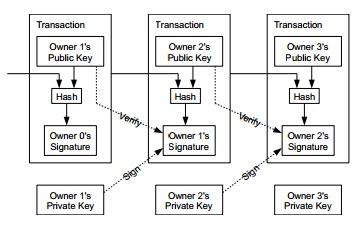
\includegraphics[scale=1]{transaction.png}
  \caption{Original Bitcoin transaction design \cite{nakamoto:bitcoin}}
\end{figure}

Thus the existence of the Bitcoin itself is governed solely by the transaction history. For our
simplified model we decided that each transaction would be a simple message indicating that Party
A has send $x$ amount of FunCoin to Party B. Thus a fundoshi transaction is a chain of such simple
messages. The authors realize that this approach is obviously not cryptographically secure. However,
the approach keeps to the main goal of design of a cryptocurrency that is easy to understand from an
outward perspective.

\subsection{Verifying Bitcoin Ownership}
Before Party B can accept payment, they must first verify that Party A has the Bitcoin to spend in the first
place. This is done by inspecting the blockchain. Party A sends Party B the pending transaction. Since every
transaction contains the history of all transactions leading up to it, Party B can check the blockchain
to ensure that the transaction history given is valid. Party B must check that the history
exists in the blockchain.

Bitcoin accomplishes validity via hashes. Party B will take the previous hash of all transactions before the pending one
and check to make sure that that hash exists in the blockchain. The actual Bitcoin implementation accomplishes
this in a space-saving manner via a merkel tree (see \ref{blockchain}).

%We may want to rethink this if we end up using a different design
Our simplified cryptocurrency would validate ownership by simply following the transaction history to the
genes of a single FunCoin. That would take care of local validity (to ensure the transaction is well formed).
From there, the receiver would check global validity by looking for the transaction history on the blockchain.



\section{Background}
In October of 2008, a white paper\cite{nakamoto:bitcoin} describing Bitcoin, a decentralized peer-to-peer electronic cash system, was published through cryptography mailing lists.

\section{OpenSSL}
The group used OpenSSL to handle most of the cryptographic functionality. OpenSSL provides a nice interface for performing digital signitures using DSA.

\bibliographystyle{abbrv}
\bibliography{report}

\end{document}
